% Subfigures: two minipage-shaped boxes under one figure, each with its
% own lettered caption, the parent captioned below — the subcaption shape.
% Synthetic: invented text, invented pictures, nothing from any private
% document. The second float checks the letters reset per parent and the
% figure counter keeps document order past a subfigured float.
\documentclass{article}
\usepackage{subcaption}

\begin{document}

\section{Paired diagrams}

A paragraph before the figure, so its separation from the text is on the
page.

\begin{figure}
\centering
\begin{subfigure}[t]{0.48\textwidth}
\centering
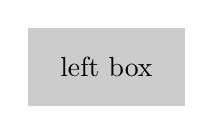
\begin{tikzpicture}
\fill[black!20] (0,0) rectangle (2,1);
\node at (1,0.5) {left box};
\end{tikzpicture}
\caption{The first invented panel.}
\end{subfigure}
\hfill
\begin{subfigure}[t]{0.48\textwidth}
\centering
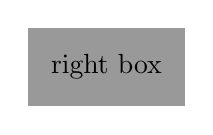
\begin{tikzpicture}
\fill[black!40] (0,0) rectangle (2,1);
\node at (1,0.5) {right box};
\end{tikzpicture}
\caption{The second invented panel.}
\end{subfigure}
\caption{Two invented panels side by side.}
\end{figure}

\begin{figure}
\centering
A plain figure body after the paired one.
\caption{The plain figure, numbered second.}
\end{figure}

A closing paragraph after both figures.

\end{document}
